% $Id: jfesample.tex,v 19:a118fd22993e 2013/05/24 04:57:55 stanton $
\documentclass[12pt]{article}

% DEFAULT PACKAGE SETUP

\usepackage{setspace,graphicx,epstopdf,amsmath,amsfonts,amssymb,amsthm,versionPO}
\usepackage{marginnote,datetime,enumitem,subfigure,rotating,fancyvrb}
\usepackage{hyperref,float}
\usepackage[longnamesfirst]{natbib}


\usdate


% These next lines allow including or excluding different versions of text
% using versionPO.sty

\excludeversion{notes}		% Include notes?
\includeversion{links}          % Turn hyperlinks on?

% Turn off hyperlinking if links is excluded
\iflinks{}{\hypersetup{draft=true}}

% Notes options
\ifnotes{%
\usepackage[margin=1in]{geometry}%
\usepackage[textwidth=1.4in,shadow,colorinlistoftodos]{todonotes}%
}{%
\usepackage[margin=1in]{geometry}%
\usepackage[disable]{todonotes}%
}

% Allow todonotes inside footnotes without blowing up LaTeX
% Next command works but now notes can overlap. Instead, we'll define 
% a special footnote note command that performs this redefinition.
%\renewcommand{\marginpar}{\marginnote}%

% Save original definition of \marginpar
\let\oldmarginpar\marginpar

% Workaround for todonotes problem with natbib (To Do list title comes out wrong)
\makeatletter\let\chapter\@undefined\makeatother % Undefine \chapter for todonotes

% Define note commands
\newcommand{\smalltodo}[2][] {\todo[caption={#2}, size=\scriptsize, fancyline, #1] {\begin{spacing}{.5}#2\end{spacing}}}
\newcommand{\rhs}[2][]{\smalltodo[color=green!30,#1]{{\bf RS:} #2}}
\newcommand{\rhsnolist}[2][]{\smalltodo[nolist,color=green!30,#1]{{\bf RS:} #2}}
\newcommand{\rhsfn}[2][]{%  To be used in footnotes (and in floats)
\renewcommand{\marginpar}{\marginnote}%
\smalltodo[color=green!30,#1]{{\bf RS:} #2}%
\renewcommand{\marginpar}{\oldmarginpar}}
%\newcommand{\textnote}[1]{\ifnotes{{\noindent\color{red}#1}}{}}
\newcommand{\textnote}[1]{\ifnotes{{\colorbox{yellow}{{\color{red}#1}}}}{}}

% Command to start a new page, starting on odd-numbered page if twoside option 
% is selected above
\newcommand{\clearRHS}{\clearpage\thispagestyle{empty}\cleardoublepage\thispagestyle{plain}}

% Number paragraphs and subparagraphs and include them in TOC
\setcounter{tocdepth}{2}

% JFE-specific includes:

\usepackage{indentfirst} % Indent first sentence of a new section.
\usepackage{jfe}          % JFE-specific formatting of sections, etc.

\newtheorem{theorem}{Theorem}[section]
\newtheorem{assumption}{Assumption}[section]
\newtheorem{proposition}{Proposition}
\newtheorem{conjecture}{Conjecture}
\newtheorem{lemma}{Lemma}[section]
\newtheorem{corollary}{Corollary}
\newtheorem{condition}{Condition}

\begin{document}

\setlist{noitemsep}  % Reduce space between list items (itemize, enumerate, etc.)
%\onehalfspacing      % Use 1.5 spacing
% Use endnotes instead of footnotes - redefine \footnote command

\title{Unemployment Insurance and the Unemployment Rate: Evidence Across U.S. Counties}

\author{Ariel Goldszmidt}



\date{}              % No date for final submission

% Create title page with no page number

\renewcommand{\thefootnote}{\fnsymbol{footnote}}

\singlespacing

\maketitle

\begin{center}\normalsize ECON 20900 \qquad Spring 2017 \end{center}


\onehalfspacing
%\setstretch{1.2}
%\singlespacing

\setcounter{footnote}{0}
\renewcommand{\thefootnote}{\arabic{footnote}}
\setcounter{page}{1}

\section{Introduction \label{sec:intro}}

The relationship between unemployment insurance (hereafter, UI) and the unemployment rate is of both theoretical and practical interest. Labor economists must concern themselves with this relationship in developing models of labor markets, while policymakers are interested in how public unemployment benefits affect the aggregate labor force.

Traditional economic reasoning suggests a simple relationship: the greater the UI (either in terms of length of benefit, average weekly payout, or both), the more utility agents derive from being unemployed, and the less incentive they have to find employment (holding the wage distribution constant). Higher UI then increases the number of workers who choose to be unemployed at a given time, increasing the steady-state unemployment level. Section \ref{subsec:theoretical} presents a formal discussion of this theoretical intuition. 

As Section \ref{subsec:empirical} shows, however, economists have encountered difficulty and dispute in empirically measuring this supposed relationship between UI and unemployment. The question presents a difficult endogeneity problem, in that unemployment-prone regions may be expected to offer more generous UI. Moreover, political debate on the social welfare consequences of UI has made the question of this relationship highly contentious. These considerations warrant further research into the relationship.

Additionally, several gaps exist in the literature. While many have recently studied the effects of UI on unemployment during the Great Recession, few have considered the effects of UI in the subsequent economic recovery, during which overall unemployment has decreased substantially to pre-Recession levels. Moreover, most recent studies of UI have considered only the maximum duration of available benefits, and not the level of weekly benefits paid. Our main contribution to the literature is to apply the method used by Hagedorn, Karahan, Manovskii, and Mitman (2015), which compares adjacent counties in different states, to study the effects of both duration and level of UI benefits on unemployment in the post-Recession U.S.

In this paper, we begin by summarizing some of the important theoretical and empirical developments made toward understanding the relationship of UI and unemployment in the past 50 years. We then propose a simple model to study the predicted relationship of UI and unemployment. Next, we detail available recent data and outline an empirical procedure to assess the model. We conclude with some preliminary results and a discussion of their implications.



\section{Literature Review \label{sec:litreview}}

We now survey some relevant theoretical and empirical work on the relationship between UI and unemployment.

\subsection{Theoretical Work \label{subsec:theoretical}}

McCall's (1970) job-search model provides an early theoretical grounding for the informal argument presented in Section \ref{sec:intro}. In McCall's model, an unemployed worker may in each period pay $c$ to draw a random wage offer $x$ from a distribution $\Phi$. The worker accepts the offer if the lifetime utility it will bring her exceeds the expected utility of waiting another period and again paying $c$ to draw a new wage offer. The reservation wage is defined as the wage offer that renders the agent indifferent between accepting and rejecting employment. It is easily verified that, all else begin equal, increasing the search cost $c$ decreases the reservation wage, leading agents to more readily and quickly accept job offers, and resulting in lower aggregate unemployment. If the individual also receives some public UI benefit $b$ in each unemployed period, the benefit functions as a negative search cost, and a larger $b$ thus results in higher unemployment.

McCall's model identifies a moral hazard problem, arguing that unemployment benefits lower unemployment by decreasing the relative cost of remaining unemployed. Chetty (2008) has developed a model in which UI raises unemployment primarily through an income effect, by providing greater liquidity to unemployed low-income households.

Albrecht and Axell (1984) expand on McCall's search model by including firm behavior in the economy, endogenizing the wage distribution. The authors find that an increase in the unemployment benefit $b$ raises the steady-state general equilibrium level of unemployment, although this effect can be offset by a shift in the wage distribution. Interestingly, the authors also determine that a selective increase in the unemployment benefit, extended only to agents who derive little utility from leisure, can in fact lower steady-state unemployment.

Davidson and Woodbury (1997) offer a further extension to the classical job-search model by considering UI benefits offered only for a finite number $T$ of periods, rather than indefinitely. The authors find that the average duration of unemployment spells is increasing in both the benefit $b$ and the maximum benefit length $T$. Further, the authors demonstrate that the welfare-maximizing level of $b$ decreases in $T$, reaching a level equal to the weekly wage when $T=32$.

Still more extensions in the literature include models with partial UI coverage (Regev 2012), wage bargaining and union-financed UI (Holmlund and Lundbord 1999), and experience rating (Mortensen 1994). In general, the intuitive prediction that more generous UI increases unemployment is supported in a wide class of theoretical models.



\subsection{Empirical Work \label{subsec:empirical}}

Despite broad agreement in the theoretical literature that UI should increase unemployment, the exact quantitative relationship has proven difficult to measure conclusively. This difficulty may be due to the substantial endogeneity in models relating unemployment to UI, discussed in Section \ref{sec:intro}. Various instruments have been used in attempt to isolate the causal effects, on both the microeconomic and macroeconomic levels.

Solon (1985) exploits a 1979 U.S. policy shift that made UI benefits taxable on sufficiently high tax returns. Solon compares 1978 and 1979 data collected by the Continuous Wage and Benefit History (CWBH) program, which surveyed UI claimants in Georgia. The author proposes a hazard-rate model of individual unemployment duration using a Weibull distribution, the parameters of which are estimated by maximum likelihood. By comparing unemployment durations of high-income claimants in the 1978 and 1979 samples, Solon concludes that the tax on UI--which amounts to a decrease in weekly benefit--resulted in a decrease of expected unemployment length from 9.6 to 8.4 weeks.

McCall (1995) studies the effect of benefit levels on receipt of UI using a logit dichotomous choice model, in which the available benefit level affects the probability of an agent taking up benefits. The author uses micro-data from the Current Population Survey's Displaced Worker Supplements (CPS DWS) for 1984-1992. Exploiting differences in UI policy across states and over time, the author uses UI claimants' state and year of filing as an instrument for exogenous variation in available benefit level. He estimates that a 1\% increase in the replacement rate (the ratio of the weekly unemployment benefit to the previous weekly wage) corresponds to a 0.1-0.3\% increase in the probability of taking up UI benefits.

Recently, much literature has analyzed the effects of extensions in the maximum length of UI benefits during the Great Recession, which reached as high as 99 weeks in some states between 2009 and 2012. Farber and Valletta (2015) consider the micro effects of these extended benefits by comparing UI-eligible and UI-ineligible individuals in the Current Population Survey data. They find that the extensions had a small negative impact on the individual unemployment exit rate. The authors estimate that the unprecedented extensions accounted for only 0.4 percentage points of the 9\% national unemployment rate seen in 2010.

Chodorow-Reich and Karabarbounis (2016) offer a macroeconomic analysis of these benefit extensions. To overcome endogeneity, the authors note that UI benefit extensions were based on real-time reports of state unemployment, which suffer from substantial measurement error. By comparing the real-time reports to later revised data, the authors isolate inter-state differences in UI benefit extensions induced by measurement error rather than differences in economic fundamentals. These measurement errors provide exogenous variation in UI benefit extension, allowing the authors to identify causal effects. They conclude that the extensions had an almost negligible impact on macroeconomic outcomes, estimating that extension of benefits from 26 to 99 weeks could increase aggregate unemployment by at most 0.3 percentage points.

Hagedorn, Karahan, Manovskii, and Mitman (2015) explore the macro effects of Great Recession-era benefit extensions with a different instrument: comparing bordering counties in different states, to isolate the exogenous state UI policy from the counties' endogenous labor market fundamentals. Their results are much larger than those elsewhere in the literature, estimating that 2.5 percentage points of unemployment in 2011 were induced by benefit extensions.


\section{Model \label{sec:model}}

Unfortunately, the models discussed in Section \ref{subsec:theoretical} do not easily produce simple closed-form equations relating the steady-state unemployment rate to the available UI benefit level and maximum benefit duration. Moreover, it is beyond the scope of this paper to construct a full theoretical model for deriving such equations. For these reasons, we look to evidence from simulated models and prior empirical work to propose a regression equation.

Sargent and Stachurski (2015) combine a version of the McCall (1970) model with a ``lake'' unemployment model to analyze the effect of UI benefits on steady-state aggregate unemployment. They use a CRRA utility function and a lognormal wage distribution, and calibrate birth, death, and separation rates to match those of the U.S. The authors then numerically simulate the steady-state unemployment rate for various levels of infinite duration $(T=\infty)$ UI benefits. Their results, shown in Figure \ref{fig:unemployment}, suggest a highly linear relationship between the unemployment rate and the benefit level.

\begin{figure}[ht!]
	\centering
	\includegraphics[width=90mm]{unemployment.png}
	\caption{Steady-state unemployment as a function of per-period UI benefit level $c$. From Sargent and Stachurski (2015). \label{fig:unemployment}}
\end{figure}

To understand the relationship of the maximal weeks of UI benefits on steady-state unemployment, we turn to Davidson and Woodbury (1997). Their model demonstrates that changing the benefit $b$ while holding $T$ constant produces essentially the same effects as holding $b$ constant while changing $T$, suggesting that $T$ should enter into the regression equation in the same functional form as $b$. However, their model notes that simultaneous changes in $b$ and $T$ can have different effects than changing each individually, suggesting that an interaction term $b\times T$ should also be included in the regression.

Moreover, it seems reasonable that each county and time period contribute some fixed effect to the unemployment rate, based on permanent local business conditions and the national economic environment. We thus arrive at the fixed-effects regression equation
\begin{equation*} \label{eq:original}
	Y_{ikt} = \beta_0 + \beta_1 b_{it} + \beta_2 T_{it} + \beta_3 b_{it} T_{it} + \boldsymbol{\gamma}'\mathbf{x}_{ikt} + a_{ik} + v_{t} + u_{ikt} + \varepsilon_{ikt},
\end{equation*}
where $Y$ is the steady-state unemployment rate, $b$ the weekly UI benefit, $T$ the maximum length of the benefit, $\mathbf{x}$ a vector of controls (discussed in Section \ref{sec:data}), $a$ a county fixed effect, $v$ a time fixed effect, $u$ a county-specific time fixed effect, and $\varepsilon$ the remaining random error, which is constructed to be uncorrelated with all other covariates and fixed effects. The subscript $i$ indicates the $i^{\text{th}}$ state, $k$ the $k^{\text{th}}$ county in the $i^{\text{th}}$ state, and $t$ the $t^{\text{th}}$ time period. Note that the $b$ and $T$ terms do not receive a $k$ subscript because UI policy is set at the state level.

We suspect that the two fixed effects $a_{ik}$ and $v_{t}$ may be correlated with the state policy terms $b_{it}$ and $T_{it}$, as UI policy is designed to extend greater benefits to consistently distressed states and to all states during prolonged periods of economic downturn. The above regression equation therefore has endogeneity.

To combat this endogeneity problem, we use the standard fixed effects approach to demean out the county and time fixed effects. We obtain
\begin{equation} \label{eq:county}
\widetilde{Y}_{ikt} = \beta_1 \widetilde{b}_{it} + \beta_2 \widetilde{T}_{it} + \beta_3 \widetilde{(bT)}_{it} + \boldsymbol{\gamma}'\widetilde{\mathbf{x}}_{ikt} + \widetilde{u}_{ikt} + \widetilde{\varepsilon}_{ikt},
\end{equation}
where $\widetilde{Y}_{ikt} = Y_{ikt} - \bar{Y}_{ik} - \bar{Y}_{t} + \bar{Y}$, and $\widetilde{b}$, $\widetilde{T}$, $\widetilde{(bT)}$, $\widetilde{\mathbf{x}}$, $\widetilde{u}$, and $\widetilde{\varepsilon}$ are similarly defined.

This model may still have endogeneity, as the demeaned county-specific time fixed effect $\widetilde{u}_{ikt}$ still impacts the demeaned unemployment rate, and therefore may be positively correlated with the demeaned UI policy terms. 

To overcome this further endogeneity, suppose counties $(i,k)$ and $(j,l)$ are adjacent. Due to their adjacency, their demeaned county-specific time fixed effects are likely quite similar, so that we assume $\widetilde{u}_{ikt} - \widetilde{u}_{jlt} = 0$. Subtracting their equations thus yields
\begin{equation} \label{eq:pair}
	\widetilde{Y}_{ikt} - \widetilde{Y}_{jlt} = \beta_1 (\widetilde{b}_{it}-\widetilde{b}_{jt}) + \beta_2 (\widetilde{T}_{it}-\widetilde{T}_{jt}) + \beta_3 \left(\widetilde{(bT)}_{it} - \widetilde{(bT)}_{jt}\right) + \boldsymbol{\gamma}'(\widetilde{\mathbf{x}}_{ikt}-\widetilde{\mathbf{x}}_{jlt}) + (\widetilde{\varepsilon}_{ikt} - \widetilde{\varepsilon}_{jlt}).
\end{equation}
This equation should not have endogeneity, as the only remaining error term, $\widetilde{\varepsilon}_{ikt} - \widetilde{\varepsilon}_{jlt}$, is a linear function of the $\varepsilon$'s, and will therefore be uncorrelated with the policy terms $\widetilde{b}_{it}-\widetilde{b}_{jt}$, $\widetilde{T}_{it}-\widetilde{T}_{jt}$, and $\widetilde{(bT)}_{it} - \widetilde{(bT)}_{jt}$, themselves linear functions of the original covariates. Note, however, that we need the strong assumption that $\widetilde{u}_{ikt} = \widetilde{u}_{jlt}$ for $(ik)$ and $(j,l)$ adjacent to reach this conclusion. The validity of this assumption is discussed in Section \ref{sec:conclusions}.


\section{Data \label{sec:data}} 

To estimate our specifications in equations (\ref{eq:county}) and (\ref{eq:pair}), county-level unemployment data for April 2016-March 2017 was obtained from the Bureau of Labor Statistics' Local Area Unemployment Statistics (BLS LAUS). The U.S. Census County Adjacency File was used to construct 1,305 unique pairs of adjacent counties in different states. These pairs are shown in Figure \ref{fig:countypair}.

\begin{figure}[ht!]
	\centering
	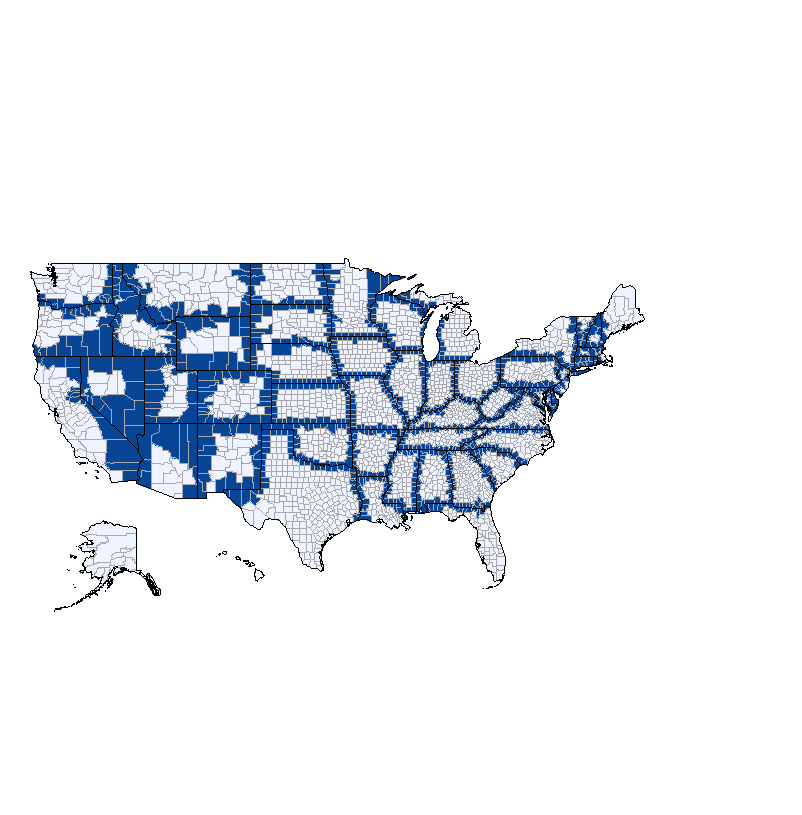
\includegraphics[width=100mm]{CountyPairs.pdf}
	\caption{Pairs of adjacent U.S. counties in different states, highlighted in blue. \label{fig:countypair}}
\end{figure}

Data on average weekly UI benefit paid in each month for each of the state and the District of Columbia was taken from U.S. Department of Labor Monthly Program and Financial Data. Data on the maximum length of UI benefits in each state and D.C. per month was obtained from the Center on Budget and Policy Priorities (CBPP) and the Congressional Research Service (CRS).

Some variables should be controlled for in our regressions. To control for broad economic welfare, we include annualized state quarterly per capita income in our regression, using data from the Bureau of Economic Analysis (BEA). Further, to account for the generosity of different UI programs, we include a ``compensation ratio'' term in the regression, which is calculated as the ratio of weeks of UI claimed to weeks of UI paid for each month and state. This ratio is calculated using the U.S. Department of Labor Monthly Program and Financial Data.

It would also be valuable to control for other factors, such as business conditions, race, and age in different areas. Unfortunately, measurements of such variables on the state and county levels are not available on time scales smaller than one year. The effects of these factors would therefore be indistinguishable from county fixed effects in our model, so we are unable to include them.

Summary statistics for our panel of counties is shown in Table \ref{tab:summary}.

\begin{table}[!htbp] \centering 
	\small
	\caption{Summary statistics for county panel data.} 
	\label{tab:summary} 
	\begin{tabular}{@{\extracolsep{5pt}}lccccc} 
		\\[-1.8ex]\hline 
		\hline \\[-1.8ex] 
		Variable & \multicolumn{1}{c}{Mean} & \multicolumn{1}{c}{St. Dev.} & \multicolumn{1}{c}{Min} & \multicolumn{1}{c}{Max} \\ 
		\hline \\[-1.8ex] 
		Unemployment rate & 5.266\% & 2.054\% & 1.345\% & 27.339\% \\ 
		Average weekly benefit & \$325.83 & \$67.67 & \$200.68 & \$541.74 \\ 
		Maximum weeks of benefit & 23.445 & 4.815 & 12 & 30 \\ 
		Compensation ratio & 85.237\% & 15.459\% & 56.833\% & 222.265\% \\ 
		Income per capita & \$46,824 & \$6,006 & \$35,639 & \$76,524 \\ 
		\hline \\[-1.8ex] 
	\end{tabular} 
\end{table} 

\section{Results \label{sec:results}}

To confirm that the fixed effect specification presented in section \ref{sec:model} is appropriate, we first ran a Hausman test on the null hypothesis that the equivalent random effects estimator is consistent. The test returned a chi-squared statistic value of 285.8 on 5 degrees of freedom, for a p-value less than $2.2\time 10^{-16}$. This result gives strong evidence that the random effects estimator in inconsistent for our purpose, and that the fixed effects estimator is to be preferred.

Following this test, we calculated the fixed effect estimator, first using equation (\ref{eq:county}) and a panel of 3,141 counties, and then using equation (\ref{eq:pair}) and a panel of 1,305 unique pairs of adjacent counties in different states. The results are shown in Table \ref{tab:results}.

\begin{table}[!htbp] \centering 
	\small
	\caption{Fixed effects estimates using equations (\ref{eq:county}) and (\ref{eq:pair}).} 
	\label{tab:results} 
	\begin{tabular}{@{\extracolsep{5pt}}lcc} 
		\\[-1.8ex]\hline 
		\hline \\[-1.8ex] 
		& \multicolumn{2}{c}{Specification} \\ 
		\cline{2-3} 
		\\[-1.8ex] & (1) & (2)\\ 
		\hline \\[-1.8ex] 
		Weekly benefit $b$ & $-$0.019 & $-$0.025 \\ 
		& (0.005) & (0.005) \\ 
		& & \\ 
		Maximum weeks of benefit $T$ & 0.194 & 0.067 \\ 
		& (0.059) & (0.074) \\ 
		& & \\ 
		Interaction $bT$ & 0.001 & 0.001 \\ 
		& (0.0002) & (0.0002) \\ 
		& & \\ 
		Compensation ratio & 0.004 & 0.005 \\ 
		& (0.0004) & (0.0004) \\ 
		& & \\ 
		Income per capita & $-$0.0002 & 0.0001  \\ 
		& (0.00004) & (0.00004) \\ 
		& & \\ 
		\hline 
		\hline \\[-1.8ex] 
		\multicolumn{3}{l}{\footnotesize \textit{Notes}: Column (1) calculated from panel of 3,141 counties over 12}\\
		\multicolumn{3}{l}{\footnotesize months, column (2) calculated from panel of 1,305 border county pairs} \\
		\multicolumn{3}{l}{\footnotesize over 12 months. Unemployment rate and compensation ratio measured} \\
		\multicolumn{3}{l}{\footnotesize in percentage points. Weekly benefit measured in dollars per week,} \\
		\multicolumn{3}{l}{\footnotesize income per capita measured in dollars per quarter. Panel-corrected} \\
		\multicolumn{3}{l}{\footnotesize clustered standard errors shown in parentheses.} \\
		\end{tabular} 
\end{table} 

All estimates shown are significant at the 1\% level, except for the coefficient on the maximum weeks of benefit $T$ in specification (\ref{eq:pair}), which is not even significant at the 10\% level.

One of the most interesting results is that the coefficient on the weekly benefit $b$ is negative under both specifications, suggesting that, all else held constant, providing an average of \$50 more per week would decrease the unemployment rate by about 1 percentage point. However, we notice that the coefficient on the interaction term $bT$ is a positive 0.001. It is straightforward to calculate that in a state providing around 20 weeks at most of UI, this interaction would cancel out the negative effect of the weekly benefit $b$, and in states providing more than 20 weeks, increasing the weekly benefit would raise the unemployment rate.

It is also interesting to note the differences between the results of the county specification (\ref{eq:county}) and the border county pair specification (\ref{eq:pair}). The estimated coefficient on the weekly benefit $b$ in specification (\ref{eq:pair}) is more negative than corresponding estimate in specification (\ref{eq:county}), suggesting that the fixed effects model ran on specification (\ref{eq:county}) underestimates the negative effect of an increased weekly benefit on the unemployment rate. Looking at the magnitudes of the different estimates, and noting that both specifications estimate the coefficient on the interaction term to be $0.001$, we see that the estimates in specification (\ref{eq:county}) suggest that increasing the weekly benefit will decrease unemployment in states where the maximum duration of benefit is at most 19 weeks, while the estimates in specification (\ref{eq:county}) suggest that increasing the weekly benefit will decrease unemployment in states where the maximum duration of benefit is as high as 25 weeks.

The estimated coefficient on the maximum weeks of benefit $T$ also differs greatly between the two specifications. The estimate in specification (\ref{eq:county}) is quite large, suggesting that increasing the maximum duration of benefits by just 5 weeks would increase unemployment by 1 percentage point. The estimate in specification (\ref{eq:pair}) is not significantly different from 0, but the point estimate suggests that it would take an increase of 15 weeks in the maximum duration of benefits to raise unemployment by 1 percentage point. We suspect, however, that both estimates may be unreliable, as our data has very little variation in the maximum length of benefits, both across states and and over time.

\section{Conclusions \label{sec:conclusions}}

The results in section \ref{sec:results} suggests that simply using a fixed effects estimator on a panel of counties to assess the relationship of UI and unemployment rate tends to overstate the extent to which UI can raise unemployment, likely due to the endogeneity problem that U.S. policies extend greater UI benefits to high-unemployment areas. Fixed effects estimation on pairs of adjacent counties in different states suggests a much smaller positive relationship between maximum weeks of benefits and the unemployment rate, and a stronger negative relationship between weekly benefit and the unemployment rate. Estimation on border county pairs seems to correct for some of the endogeneity in equation (\ref{eq:county}), and likely gives estimates that are closer to the true causal relationships.

Corroborating the results of other recent literature, we find that increasing the maximum duration of UI benefits can indeed substantially increase the unemployment rate. Our point estimate of this effect is even higher than that found by Hagedorn, Karahan, Manovskii, and Mitman (2015), who estimate that an increase of one week in maximum duration of benefits causes about a 0.03 percentage point increase in the unemployment rate. We note, however, that our estimate of this effect has too a large standard error to be taken as a precise measurement, and may be unreliable due to a lack of variation in maximum duration of benefit in our data.

Our results also have significant implications for UI policy. By simultaneously analyzing the effects of average weekly benefit and maximum duration of benefits on the unemployment rate, we estimate that increasing average weekly benefit can actually decrease the unemployment rate in states where the maximum duration of benefits is under 25 weeks. We would thus advise policymakers that lower duration, higher benefit UI policies result in lower unemployment than higher duration, lower benefit policies. The intuition behind such advice is that lower duration, higher benefit policies may encourage unemployed individuals to search more intensely for new work, and provide them with enough financial liquidity to do so. In contrast, higher duration, lower benefit policies may leave the unemployed with less financial liquidity to support an intense search, and encourage complacency with longer spells of unemployment.

Many improvements to our empirical analysis can be made in the future. First, more advanced statistical methods could be used to assess the degree of endogeneity in equation (\ref{eq:county}) and determine the extent to which equation (\ref{eq:pair}) corrects for this endogeneity. Such methods will give a better sense of how much closer the border county pair specification results are to the true causal relationships. Additionally, the assumption in section \ref{sec:model} that adjacent counties have similar county- and time-specific fixed effects must be rigorously assessed, as the validity of our border county pair model depends on this assumption. One way to assess this assumption would be to gather panel data of county demographics and local business conditions over time, and measure whether adjacent counties are indeed comparable over time.

More data would also be valuable for this analysis. To truly measure the effect of UI policies on county unemployment, we should gather data on UI payouts in each county, rather than relying on state-level aggregates, as counties within a state may differ systematically in their receipt and level of UI benefits. Obtaining county-level data on per-capita income, hiring, and other government benefit programs over time would also be useful for adding more controls to our models, to better isolate the effects of UI. Lastly, performing similar analyses on different time periods in U.S. history, both in and out of recession, would let us assess whether the causal relationship between UI and unemployment has changed or remained constant over time.


\clearpage

% Bibliography.

\bibliographystyle{jfe}
% \bibliography{RHSbib}
\begin{thebibliography}{9}
	\singlespacing
	
	\bibitem{latexcompanion} 
	McCall, J. J.
	``Economics of Information and Job Search.'' 1970.
	\textit{The Quarterly Journal of Economics}, \textbf{84} (1): 113-126.
	
	\bibitem{latexcompanion} 
	Chetty, Raj.
	``Moral Hazard versus Liquidity and Optimal Unemployment Insurance.'' 2008.
	\textit{Journal of Political Economy}, \textbf{116} (2): 173-234.
	
	\bibitem{latexcompanion} 
	Albrecht, James W. and Bo Axell.
	``An Equilibrium Model of Search Unemployment.'' 1984.
	\textit{Journal of Political Economy}, \textbf{92} (5): 824-840.
	
	\bibitem{latexcompanion} 
	Davidson, Carl and Stephen A. Woodbury.
	``Optimal unemployment insurance.'' 1997.
	\textit{Journal of Public Economics}, \textbf{64}: 359-387.
	
	\bibitem{latexcompanion} 
	Regev, Tali.
	``Unemployment compensation under partial program coverage.'' 2012.
	\textit{Labour Economics}, \textbf{19}: 888-897.
	
	\bibitem{latexcompanion} 
	Holmlund, Bertil and Per Lundborg.
	``Wage bargaining, union membership, and the organization of unemployment insurance.'' 1999.
	\textit{Labour Economics}, \textbf{6}: 397-415.
	
	\bibitem{latexcompanion} 
	Mortensen, Dale.
	``Reducing Supply-Side Disincentives to Job Creation.'' 1994.
	In \textit{Reducing Unemployment: Current Issues and Policy Options}, Federal Reserve Bank of Kansas City, 189-219.
	
	\bibitem{latexcompanion} 
	Solon, Gary.
	``Work Incentive Effects of Taxing Unemployment Benefits.'' 1985.
	\textit{Econometrica}, \textbf{53} (2): 397-415.
	
	\bibitem{latexcompanion} 
	McCall, Brian P.
	``The Impact of Unemployment Insurance Benefit Levels on Recipiency.'' 1995.
	\textit{Journal of Business \& Economic Statistics}, \textbf{13} (2): 189-198.
	
	\bibitem{latexcompanion} 
	Farber, Henry S. and Robert G. Valletta.
	``Do Extended Unemployment Benefits Lengthen Unemployment Spells? Evidence from Recent Cycles in the U.S. Labor Market.'' 2015.
	\textit{The Journal of Human Resources}, \textbf{50} (4): 873-909.
	
	\bibitem{latexcompanion} 
	Chodorow-Reich, Gabriel and Loukas Karabarbounis.
	``The Limited Macroeconomic Effects of Unemployment Benefit Extensions.'' 2016.
	Federal Reserve Bank of Minneapolis Working Paper.
	
	\bibitem{latexcompanion} 
	Hagedorn, Marcus, Fatih Karahan, Iourii Manovskii, and Kurt Mitman.
	``Unemployment Benefits and Unemployment in the Great Recession: The Role of Macro Effects.'' 2015.
	\emph{Federal Reserve Bank of New York Staff Reports}, no. 646.
	
	\bibitem{latexcompanion} 
	Sargent, Thomas and John Stachurski.
	``A Lake Model of Employment and Unemployment.'' 2015.
	In \emph{Quantitative Economics with Python}.
	
\end{thebibliography}


 

\end{document}
